\documentclass[12pt,fleqn]{article}\usepackage{../../common}
\begin{document}
Yapay Sinir Ağları (Neural Networks)

YSA'ları anlamak için onların temel taşı olan tek nöron'u görmemiz lazım. 

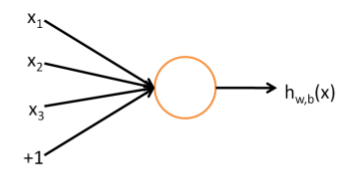
\includegraphics[height=3cm]{mlp_03.png}

Üstteki resimde üç girdisi ve tek çıktısı olan bir nöron görüyoruz. Girdi
olarak $x_1,x_2,x_3$ ve çıktı olarak bir fonksiyon hesabı. Literatürde
üstteki yapıya perseptron (perceptron) ismi de veriliyor. Eğer 0/1,
evet/hayır türünde çıktıları modellemek istersek bu fonksiyon çoğunlukla
sigmoid fonksiyonu olarak seçilir. Yani

$$ h (x) = f(w^Tx) = f(\sum_{i=1}^{3} w_ix_i + b)$$

ve 

$$ f(z) = \frac{1}{1 + \exp(-z)}$$

ki $w$ ağırlık değerlerinin taşıyan bir vektördür. Sigmoid seçiminin bir
diğer sebebi türevinin rahat alınabilmesi. Alternatif fonksiyonlar $\tanh$
olabilirdi, ya da düzeltilmiş lineer ünite (rectified linear unit -ReLu-)
fonksiyonları. ReLu'lar YSA'ların uzantısı Derin Öğrenim'de oldukca popüler
oldu, tanımı

$$ f(z) = \max(0,z)$$

Şimdi tek nörondan çok katmanlı bir YSA nasıl oluşturulur görelim, 

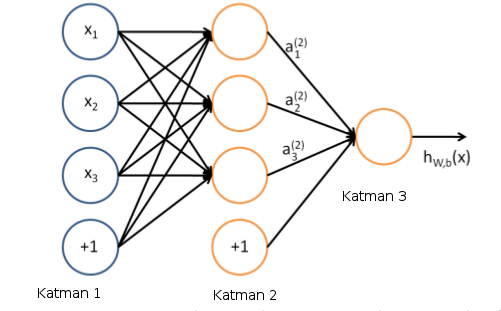
\includegraphics[height=6cm]{mlp_04.png}

Bu yapıda her $x_i$'in her nörona gittiğini görüyoruz, bu katmanlara bu
sebeple tamamen bağlanmış katman (fully-connected layer), ya da yoğun
(dense) katman deniyor. Her türlü girdi / nöron kombinasyonu çarpıldığı
için ağırlıklar bir matris içinde tutulur, ve aktivasyondan önceki vektör
basit bir matris çarpımı haline gelir, mesela 2. katman aktivasyonu $f_2$
olsun, 1. gizli katman çıktısı

$$ f_2 (W_1x + b) $$

Girdi $4 \times 1$, ağırlık $W_1$ boyutu $3 \times 4$, o zaman çarpım
$3 \times 1$ olacak, $f_2$ uygulanınca boyut değişmez (her öge üzerinde
aynı fonksiyon işletiliyor) sonuç $3 \times 1$, bu da zaten 2. katmana
giren (sonra oradan sonraki katmana çıkan) hesap. Üstteki diyagramda
yanlılık (bias) ayrı bir nöron olarak eklenmiş (bazen bu yapılmayabiliyor).

İki gizli seviyesi (hidden layer) olan bir YSA,

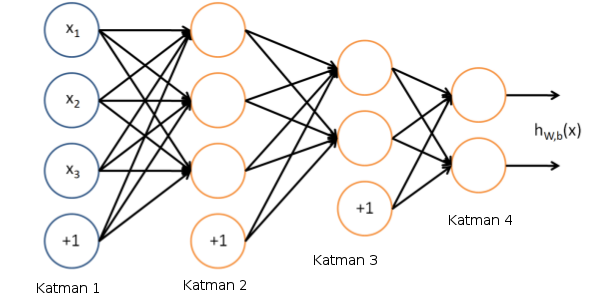
\includegraphics[height=6cm]{mlp_05.png}

Görüldüğü gibi çok seviyeli durumda bir seviyenin çıktısı bir diğer
seviyenin girdisi haline geliyor. YSA'lar denetimli (supervised) şekilde
eğitilirler. Elde $x_i,y_i$ veri noktaları vardır, ve her bir ya da çok
boyutlu $x_i$ yine bir ya da çok boyutlu $y_i$ ile eşlidir. Aynen
regresyonda olduğu gibi bu veri çiftlerini alırız ve onları en iyi temsil
eden YSA'yı eğitmek için kullanırız. Eğitim tamamlandığında $i$
katmanındaki $W_i$ ağırlıkları belli değerlere sahip olurlar, ve eldeki
``model'' bu ağırlıklardır. Yeni bir veri noktası verildiğinde o veri
noktası ağırlıklar her katmanın $W_i$'sı ile çarpılıp, toplanıp, aktivasyon
fonksiyonlarına geçilip, tüm katmanlardan bu şekilde geçirildikten sonra en
sondaki çıktı değerine erişilir.

Yanlılık taşımayan şekilde ağ yapısı görelim ve matris çarpımı ile tüm
girdileri /  çıktıları gösterelim,

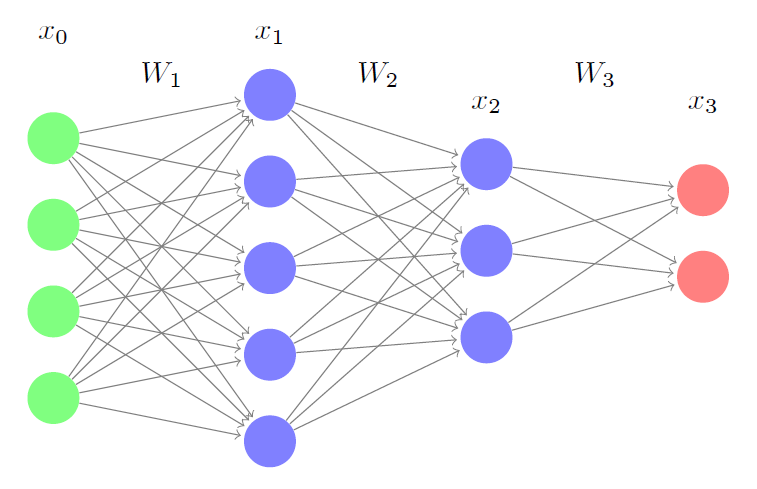
\includegraphics[width=30em]{nn_nobias.PNG}

$$ Girdi = x_0$$

$$ x_1 = f_1(W_1x_0)$$

$$ x_2 = f_2(W_2x_1)$$

$$ Çıktı = f_3(W_3x_2) $$

Aktivasyon için $f_1,f_2,f_3$ ReLu ya da sigmoid seçilebilir.

İki gizli seviyesi olan (ve yeterince sayıda nöron içeren) YSA'nın evrensel
yaklaşıklayıcı (universal approximator) olduğu iddia edilir, yani üstteki
gibi yeterince çetrefil bir YSA her türlü fonksiyonu yaklaşık olarak temsil
edebilir. İşin tarihine gidersek, ilk başta tek seviyeli YSA vardı, fakat
XOR fonksiyonunu başarılı şekilde temsil edemedi. Gizli (tek) seviyeli olan
bunu başardı.

YSA'lar imaj tanıma alanında bolca kullanılmıştır. Bir imajda, mesela sayı
tanıma uygulamasında, alttaki gibi pek çok resimler olabilir,


\includegraphics[height=5cm]{mlp_01.png}
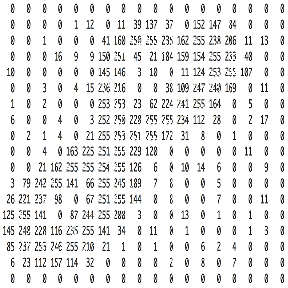
\includegraphics[height=5cm]{mlp_02.png}

Bir imaj nihayetinde o resmi temsil eden gri değerlerin olduğu bir
matristen ibarettir. YSA'ya girdi olması için matris genelde düzleştirilir,
ve tek bir vektör olarak verilir, 8x8 matris 64x1 vektörü olur, girdi 64
boyutlu bir $x_i$ çıktı ise tek boyutlu 0,1,2,..,9 gibi
etiketler.. Çoğunlukla bu tür kategorik çıktılar ikisel olarak modellenir,
0,..,9 yerine 10 öğeli bir ikisel vektör alınır, 9. öğesi 1 diğerleri 0 yapılır.

YSA'lar nasıl eğitilir? Eldeki $x_i,y_i$ çiftleri YSA'ya verilir, her $x_i$
önce tahmin için kullanılır, ve bir YSA'nın tahmin ettiğine, bir de gerçek
veriye bakılır. Bu fark, hata, YSA'nın düzeltilmesi / iyileştirilmesi için
kullanılır, burada geriye yayılım (backpropagation -backprop-) adlı bir
teknik var. YSA içinde, üstte gördüğümüz gibi, sol seviyeden başlayarak
sağa gidecek şekilde, fonksiyonlar, fonksiyonların fonksiyonları şeklinde
çetrefil bir yapı var. Backprop elde hatayı alıp YSA'daki tüm nöronların
ağırlıklarını bu hataya göre düzeltilmesini, düzelmenin ``yayılmasını''
sağlar [1,2]. Bu işlem ardı ardına, farklı her döngüde tekrarlanır, bir
süre sonra YSA eldeki veriyi en iyi temsil eden ideal bir hale
yaklaşacaktır.

Formüller ve Kod

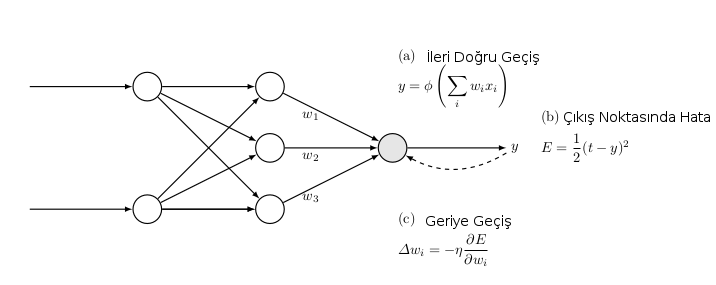
\includegraphics[width=35em]{mlp_07.png}

Backprop'un genel bir resmi üstte: a) Eğitim verisi ileri yönde (soldan
sağa) YSA'ya veriliyor, ve bu veri her nokta için, o anda sahip olunan
ağırlıklara göre bir tahmin üretiyor. b) Eğitim verisindeki beklenen ve
tahmin edilen değerler arasındaki hata hesaplanıyor c) Hata YSA'ya ``geri
yönde'' veriliyor, her ağırlık $w_i$'dan $\frac{\partial E}{\partial w_i}$
büyüklüğünün bir kısmı çıkartılıyor, bu düzeltmenin ne oranda yapıldığı
dışarıdan, önceden kararlaştırılan bir sabit $\eta$'e oranda
yapılıyor. 

Daha detaylı bir resimde gösterelim,

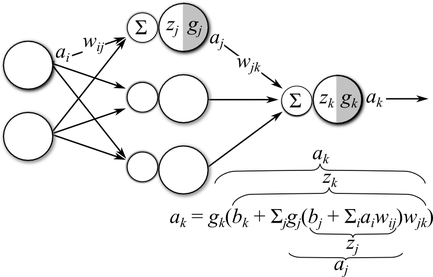
\includegraphics[width=20em]{neural-net.png}

Tek bir gizli katman var, girdi katmanı $a_i$'den gelen sinyaller $w_{ij}$
ağırlıkları ile çarpılıyor, daha önce gördüğümüz gibi bu tamamen bağlanmış
katman, çünkü tüm girdi sinyalleri her gizli katman düğümüne hep beraber
giriş yapıyorlar (tabii farklı ağırlıklar üzerinden). Devam edelim,
ağırlıklar sonrası bir de yanlılık (bias) eklenecek (resimde atlandı), ve
elde edilen $z_i = b_j + \sum_i a_i w_{ij}$. Bu 3. katmandaki aktivasyon
önceki son hal. Gizli katmandan çıkan sinyal $a_j$, bu sinyaller son
katmanda bu sefer $w_{jk}$ ağırlıkları ile çarpılıp toplanacak, $b_k$
yanlılığı eklenecek, ve sonuç $g_k$ aktivasyon fonksiyonundan geçirilip
çıktı $a_k$ haline getirilecek.

Bir YSA'yı eğitmek demek öyle bir parametre demeti $\theta = (W,b)$
bulmaktır ki ağın hatası en minimal seviyede olsun. Çoğunlukla bu hata
hedef (eğitim) çıktısı $t_k$ ile ağın en son ağırlıklara göre kendi
hesapladığı $a_k$ fark karelerinin toplamı üzerinden hesaplanır. 

$$ E = \frac{1}{2}  \sum_k (a_k - t_k)^2$$

Çıktı katmanının hata fonksiyonu üzerinde direk etkisi olduğu için bu
parametreler için gradyanı hesaplamak oldukca kolay, 

$$ \frac{\partial E}{\partial w_{jk}} = \frac{1}{2} \sum_k (a_t - t_k)^2$$

$$ = (a_k-t_k) \frac{\partial }{\partial w_{jk}} (a_k-t_k)$$

Bu türevde Zincirleme Kanununu kullandık. Dikkat edersek toplama operatörü
kayboldu, bunun sebebi $j$'inci düğüme göre türev alıyor olmamız o yüzden
$j$'inci haricinde tüm diğer parametreler türevde sıfırlanıyor, toplamdan
geriye tek bir terim kalıyor. $t_k$'in türevi de sıfır çünkü içinde
$w_{jk}$'ye bağlı hiçbir değişken yok ($t_k$ dışarıdan verilen eğitim
verisi sonuçta, çoğu durum için sabit sayılabilir). Ayrıca $a_k =
g(z_k)$ olduğunu hatırlayalım. O zaman 

$$  
\frac{\partial E}{\partial w_{jk}}  = 
(a_k-t_k)  \frac{\partial}{\partial w_{jk}} a_k 
$$

$$  
= (a_k-t_k)  \frac{\partial}{\partial w_{jk}} g_k(z_k) 
$$

$$  
= (a_k-t_k)g_k'(z_k)\frac{\partial}{\partial w_{jk}} z_k 
\mlabel{1}
$$

Yine Zincirleme Kanununu kullandık. Şimdi hatırlayalım ki
$z_k=b_j+\sum_j g_j(z_j)w_{jk}$, yani
$\frac{\partial z_k}{\partial w_{jk}} = g_j(z_j) = a_j$, demek ki

$$  
\frac{\partial E}{\partial w_{jk}} =  (a_k-t_k)g_k'(z_k) a_j
$$

Bu üç terimin çarpımı, birincisi ağ çıktısı ``tahmini'' ile hedef değerinin
farkı, diğeri çıktı katmanının aktivasyon fonksiyonunun türevi. Üçüncüsü
gizli katmandaki $j$'inci düğümün aktivasyon çıktı değeri. Bu üçlü çarpımı
kısaltılmış şekilde göstermek için $k$ indisi için $\delta_k$ değişkeni
tanımlayabiliriz, 

$$ \delta_k = (a_k-t_k)g_k'(z_k)$$

O zaman 

$$ \frac{\partial E}{\partial w_{jk}} =  \delta_k a_j $$

$\delta_k$ değişkeni hatanın çıktı aktivasyonunden geriye doğru
filtrelenmiş hali olarak görülebilir, yani bir tür hata sinyali olarak
alınabilir. Kabaca belirtmek gerekirse üstteki formül her $w_{jk}$'nin
nihai hataya ne kadar ek yaptığını belirtir. Bu sebeple, eğitim sırasında,
bu hataların tersi yönde gidilmelidir ki hata daha azalsın. 

$$ w_{jk} \leftarrow w_{jk} - \eta  \frac{\partial E}{\partial w_{jk}} $$

Çıktı Katman Yanlılığı, $b_k$

Yanlılık için $w_{jk}$'ye benzer bir yaklaşımı takip ediyoruz, tek fark
(1)'deki 3. terim şöyle, 

$$ 
\frac{\partial }{\partial b_k} z_k = 
\frac{\partial }{\partial b_k} \big[ b_k + \sum_j g_j(z_j) \big] = 1 
$$

ve sonuç olarak alttaki gradyanı elde ediyoruz, 

$$  \frac{\partial E}{\partial b_k} (a_k-t_k) g_k'(z_k)(1)$$

$$ = \delta_k$$

Yani yanlınlık gradyanı sadece çıktı ünitelerinin geriye yayılmış hali. Bu
mantıklı aslında çünkü yanlılığın aktivasyon üzerindeki ağırlığı hep 1'e
eşit, ileri doğru giden sinyal ne olursa olsun. Bu sebeple yanlılık
gradyanı ileri giden sinyalden hiç etkilenmiyor, sadece hatanın kendisinden
etkileniyor. 

Gizli Katman Ağırlıklarının Gradyanı

Bu katmanın nihai hata üzerinde etkisi dolaylı olduğu için gizli katman
ağırlıkları $w_{ij}$ için gradyanları hesaplamak biraz daha zor. Fakat
hesaba yine aynı şekilde başlıyoruz, 

$$ \frac{\partial E}{\partial w_{ij}} = 
\frac{1}{2} \sum_k (a_k-t_k)^2
$$

$$ = \sum_k (a_k-t_k) \frac{\partial }{\partial w_{ij}} a_k$$

Dikkat edersek toplam operatörü bu sefer kaybolmadı, çünkü katmanların tam
bağlı olması sebebiyle, her gizli katman ünitesinden çıkan sonuç her çıktı
katmanındaki üniteyi etkiliyor. Devam edersek, ve $a_k = g_k(z_k)$
olmasından hareketle,

$$ 
\frac{\partial E}{\partial w_{ij}} = 
\sum_k (a_k-t_k) \frac{\partial }{\partial w_{ij}} g_k(z_k)
$$

$$ 
= \sum_k (a_k-t_k) g_k'(z_k) \frac{\partial }{\partial w_{ij}}z_k \mlabel{2}
$$

Yine Zincirleme Kanununu kullandık. Evet, şimdi işler biraz daha
karmaşıklaşacak. Üstteki formüldeki üçüncü terimde olan kısmi türeve
bakarsak, bu türev $w_{ij}$'e göre ama türevi alınan $z_j$ $j$ indisine
bağlı. Şimdi ne yapacağız? $z_k$'yi açınca içinde alt fonksiyonlar olduğunu
görüyoruz, 

$$ z_k = b_k + \sum_j a_j w_{jk}$$

$$ = b_k + \sum_j g_j(z_j) w_{jk}$$

$$ = b_k + \sum_j g_j (b_i + \sum_i z_i w_{ij})w_{jk}  $$

Üstteki son denklemdeki son terime göre $z_k$ sadece dolaylı olarak
$w_{ij}$'ye bağlı. Bu ayrıca demektir ki Zincirleme Kanununu kullanarak
$\frac{\partial z_k}{\partial w_{ij}}$'i hesaplayabiliriz. Türetimin belki
de en püf noktalı yeri burası.. 

$$ 
\frac{\partial z_k}{\partial w_{ij}} =
\frac{\partial z_k}{\partial a_j}\frac{\partial a_j}{\partial w_{ij}}
$$

$$ = \frac{\partial }{\partial a_j} a_j w_{jk} \frac{\partial a_j}{\partial w_{ij}}$$

$$ = w_{jk} \frac{\partial a_j}{\partial w_{ij}}$$

$$ = w_{jk} \frac{\partial g_j(z_j)}{\partial w_{ij}}$$

$$ = w_{jk}g_k'(z_j)\frac{\partial z_j}{\partial w_{ij}}$$

$$ = w_{jk}g_j'(z_j) \frac{\partial }{\partial w_{ij}}(b_i + \sum_i a_iw_{ij})$$

$$ = w_{jk}g_j'(z_j)a_i$$

Eğer üstteki formülü (2)'deki $z_k$'ye koyarsak, $\frac{\partial E}{\partial w_{ij}}$ 
için şunu elde ederiz, 

$$ \frac{\partial E}{\partial w_{ij}} = 
\sum_k (a_k-t_k)g_k'(z_k)w_{jk}g_j'(z_j)a_i
$$

$$ g_j'(z_j)a_i \sum_k (a_k-t_k)g_k'(z_k)w_{jk} $$

$$ = a_ig_j'(z_j) \sum_k \delta_k w_{jk} $$

Gizli katman yanlılığının gradyanı için Zincirleme Kanunu ile 
$\frac{\partial z_k}{\partial b_i}$ hesabını yapmak lazım. 

$$ \frac{\partial z_k}{\partial b_i} = 
w_{jk}g_j'(z_j) \frac{\partial z_j}{\partial b_i} 
$$

$$ = w_{jk}g_j'(z_j) \frac{\partial }{\partial b_i} (b_i + \sum_i a_iw_{ij})$$

$$ = w_{jk}g_j'(z_j) (1)$$

bunun sonucu

$$ \frac{\partial E}{\partial b_i} = g_j'(z_j) \sum_k \delta_k w_{jk} $$

$$ = \delta_j $$

Özet olarak YSA eğitimi için yapılan hesaplar şunlar: 

1. İleri yönde sinyalleri girdiden çıktıya doğru hesapla

2. Tahmin $a_k$ ve hedef $t_k$'ye göre hata $E$'yi hesapla

3. Hatayı önceki katmanlardaki ağırlıklar ve aktivasyon fonksiyonlarının
gradyanlarına göre geriye doğru yay.

4. Parametreleri her parametrenin gradyanı için $\theta \leftarrow \theta -
\eta \frac{\partial E}{\partial \theta}$ şeklinde güncelle.

Kodlar

Alttaki kod [3] baz alınarak yazıldı. Bu arada hem gizli, hem çıktıdaki
aktivasyonlar $g_k,g_j$, ya da hata $E$ hesabında farklı seçimler
yapılabilir. Mesela [3] üstte belirttiğimiz gibi hata hesaplıyor ama
[2]'deki hata

$$ E = -\frac{1}{N} \sum_n \sum_i y_{n,i} \log \hat{y}_{n,i}$$

ile hesaplanıyor. Her iki kod çıktı aktivasyonu için ``softmax'' denen
fonksiyon kullanıyor. Softmax 0/1 kararı yapan lojistik fonksiyonun 2'den
fazla çıktı boyutu için genellenmiş halidir, yani iki seçimden biri yerine
K seçimden biri için kullanılır, ve

$$ \sigma(z)_j = \frac{e^{z_j}}{\sum_{k=1}^{K} e^{z_k}}$$

ile hesaplanır, $z$ vektöründeki herhangi bazı reel değerleri ``ezerek''
$\sigma(z)$ vektörü içinde toplamı 1 olacak değerlere çevirir. 

Alttaki kod gizli katman aktivasyonu için sigmoid kullanmış. 

\inputminted[fontsize=\footnotesize]{python}{mlp.py}

\begin{minted}[fontsize=\footnotesize]{python}
from sklearn.cross_validation import train_test_split
from sklearn import datasets
import mlp

def generate_data():
    np.random.seed(0)
    X, y = datasets.make_moons(200, noise=0.20)
    return X, y

one_hot = lambda x, K : np.array(x[:,None] == np.arange(K)[None, :], dtype=int)

X, y = generate_data()
y2 = one_hot(y, 2)
print X.shape, y2.shape
X_train, X_test, y_train, y_test = train_test_split(X, y2, test_size=0.2,random_state=0)
print X_train.shape, y_train.shape
print X_test.shape, y_test.shape
net = mlp.mlp(X_train,y_train,2)
print net.earlystopping(X_train,y_train,X_test,y_test,0.1)
\end{minted}

\begin{verbatim}
(200, 2) (200, 2)
(160, 2) (160, 2)
(40, 2) (40, 2)
Stopped 2.86548233378 2.86551829438 2.86620503073
Out[1]: 
2.8654823337797608
\end{verbatim}

\begin{minted}[fontsize=\footnotesize]{python}
def predict(x): 
    inputs2 = np.concatenate((x,-np.ones((np.shape(x)[0],1))),axis=1)
    outputs = net.mlpfwd(inputs2)
    return np.where(outputs>0.5,1,0)

def plot_decision_boundary(XX, yyy):
    # Set min and max values and give it some padding
    x_min, x_max = XX[:, 0].min() - .5, XX[:, 0].max() + .5
    y_min, y_max = XX[:, 1].min() - .5, XX[:, 1].max() + .5
    h = 0.01
    # Generate a grid of points with distance h between them
    xx, yy = np.meshgrid(np.arange(x_min, x_max, h), np.arange(y_min, y_max, h))
    # Predict the function value for the whole gid
    Z = predict(np.c_[xx.ravel(), yy.ravel()])
    Z = Z.argmax(axis=1)
    Z = Z.reshape(xx.shape)
    # Plot the contour and training examples
    plt.contourf(xx, yy, Z, cmap=plt.cm.Spectral)
    yyy = yyy.argmax(axis=1)
    XX1 = XX[yyy==0]; XX2 = XX[yyy==1]
    plt.scatter(XX1[:, 0], XX1[:, 1], color='blue')
    plt.hold(True)
    plt.scatter(XX2[:, 0], XX2[:, 1], color='red')

plot_decision_boundary(X, y2)
plt.savefig('mlp_06.png')
\end{minted}

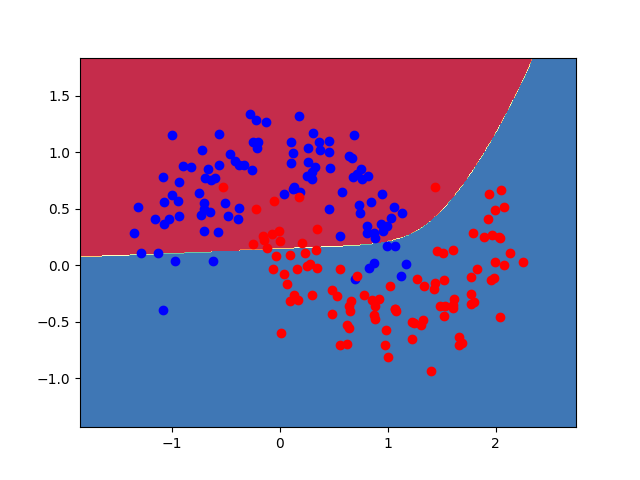
\includegraphics[width=20em]{mlp_06.png}

Alttaki alternatif bir kod, bu kod [2]'yi baz alıyor, YSA ile 0/1
regresyonu yapacak, gizli katman aktivasyonu için $\tanh$
kullanılmış. Karar sınırları grafikleniyor.

\inputminted[fontsize=\footnotesize]{python}{mlp2.py}

\begin{minted}[fontsize=\footnotesize]{python}
import mlp2
X, y = mlp2.generate_data()

model = mlp2.build_model(X, y, 3, print_loss=True)
mlp2.plot_decision_boundary(lambda x:predict(model,x), X, y)
plt.title('YSA')
plt.savefig('mlp_08.png')
\end{minted}

\begin{verbatim}
Loss after iteration 0: 0.432387
Loss after iteration 1000: 0.068947
Loss after iteration 2000: 0.068883
Loss after iteration 3000: 0.070752
Loss after iteration 4000: 0.070748
Loss after iteration 5000: 0.070751
Loss after iteration 6000: 0.070754
Loss after iteration 7000: 0.070756
Loss after iteration 8000: 0.070757
Loss after iteration 9000: 0.070758
Loss after iteration 10000: 0.070758
Loss after iteration 11000: 0.070758
Loss after iteration 12000: 0.070758
Loss after iteration 13000: 0.070758
Loss after iteration 14000: 0.070758
Loss after iteration 15000: 0.070758
Loss after iteration 16000: 0.070758
Loss after iteration 17000: 0.070758
Loss after iteration 18000: 0.070758
Loss after iteration 19000: 0.070758
\end{verbatim}

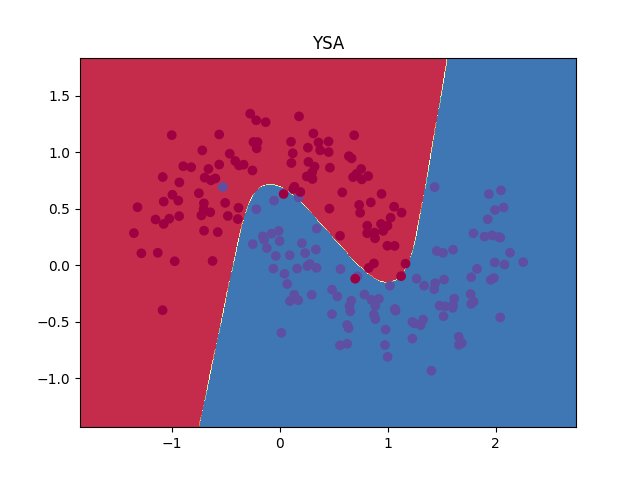
\includegraphics[width=30em]{mlp_08.png}

Karşılaştırmak için lojistik regresyon kullanalım, ve aynı karar
sınırlarını grafikleyelim,

\begin{minted}[fontsize=\footnotesize]{python}
clf = linear_model.LogisticRegressionCV()
clf.fit(X, y)
mlp2.plot_decision_boundary(lambda x: clf.predict(x), X, y)
plt.title('Lojistik Regresyon')
plt.savefig('mlp_09.png')
\end{minted}

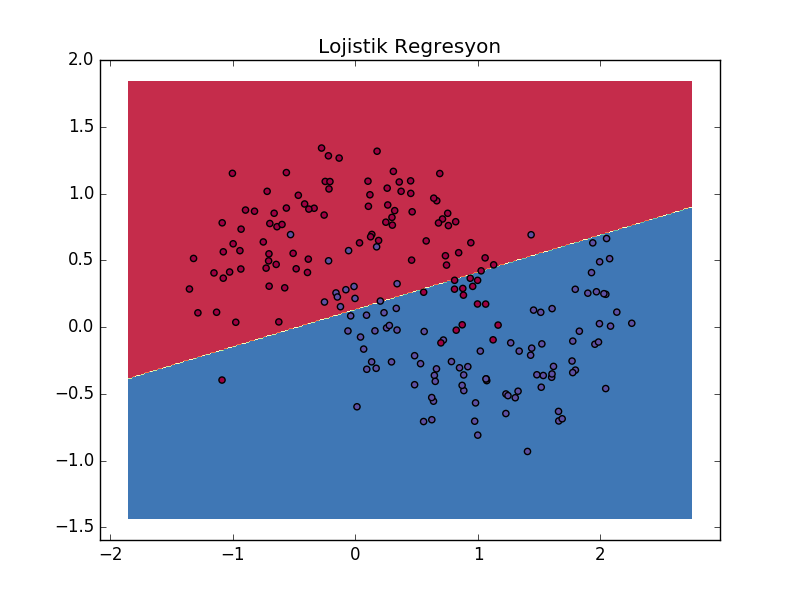
\includegraphics[width=30em]{mlp_09.png}

Görüldüğü gibi karar sınırı daha basit, kıyasla YSA çok daha esnek bir
şekilde ayrım yapabiliyor. 

Aktivasyon Fonksiyonları

Biraz once ReLu'dan bahsettik, $tanh$ yerine kullanilabilir. Bir diger
fonksiyon sigmoid. Bu fonksiyonlarin tipik grafikleri alttadir. 

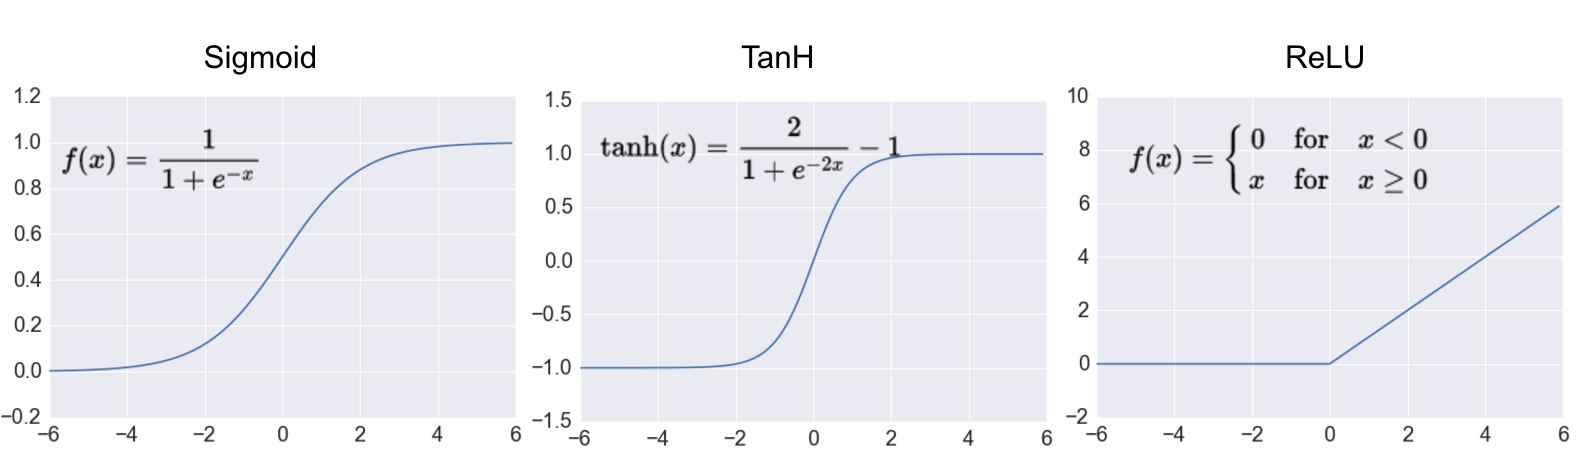
\includegraphics[width=35em]{mlp_10.png}

Kaynaklar

[1] Stansbury, {\em Derivation: Error Backpropagation \& Gradient Descent for Neural Networks}, \url{https://theclevermachine.wordpress.com/2014/09/06/derivation-error-backpropagation-gradient-descent-for-neural-networks/}

[2] Britz, {\em Implementing a Neural Network from Scratch in Python - An Introduction}, \url{http://www.wildml.com/2015/09/implementing-a-neural-network-from-scratch/}

[3] Marsland, {\em Machine Learning - An Algorithmic Approach}

\end{document}
